\section{Case study}
\label{sec:case_study}

\begin{table*}[t]
    \centering
    \begin{tabular}{c c c c c c}
    \hline
        Case & Categories & Controllers & Properties & Behaviors  \\ 
        \hline
        D1(R) & Conflicted config & Deployment + Kubelet & Liveness & Scheduling and evicting pods infinitely  \\ 
        H1(R) & Lack of context & HPA + App CPU changes & Safety & HPA is agnostic to app  \\ 
        H2(R) & Conflicted config & HPA + Deployment & Safety & Sub-optimal scaling behavior  \\ 
        H3(R) & Lack of context & HPA + Node reachability & Safety & Semantically wrong avg CPU util (reachability vs healthiness)  \\ 
        S1 & Conflicted config & Descheduler + Daemonset & Liveness & High utilization(scheduler) <-> Low utilization(descheduler) \\ 
        S2(R) & Conflicted config & Scheduler + Descheduler & Liveness & Deployment preference <-> Violation in maxSkew \\ 
        S3(R) & Conflicted config & Scheduler & Liveness & Two pod spread constraints are conflicted each other  \\ 
        S5 & Conflicted config & Scheduler & Safety & Pods are scheduled to one node, because of skewed preference  \\ 
        S6(R) & Lack of feature & Scheduler & Safety & Scheduler is not able to adjust skewed placement  \\ 
        S7(R) & Lack of context & Scheduler + Kubelet & Liveness & Scheduler includes NotReady node for maxSkew calculation  \\ 
        \hline
    \end{tabular}
    \caption{Summary of multi-controller failure cases. Reproduced cases are marked with (R).}
    \label{table:summary}
\end{table*}


\begin{figure}[h]
    \centering
    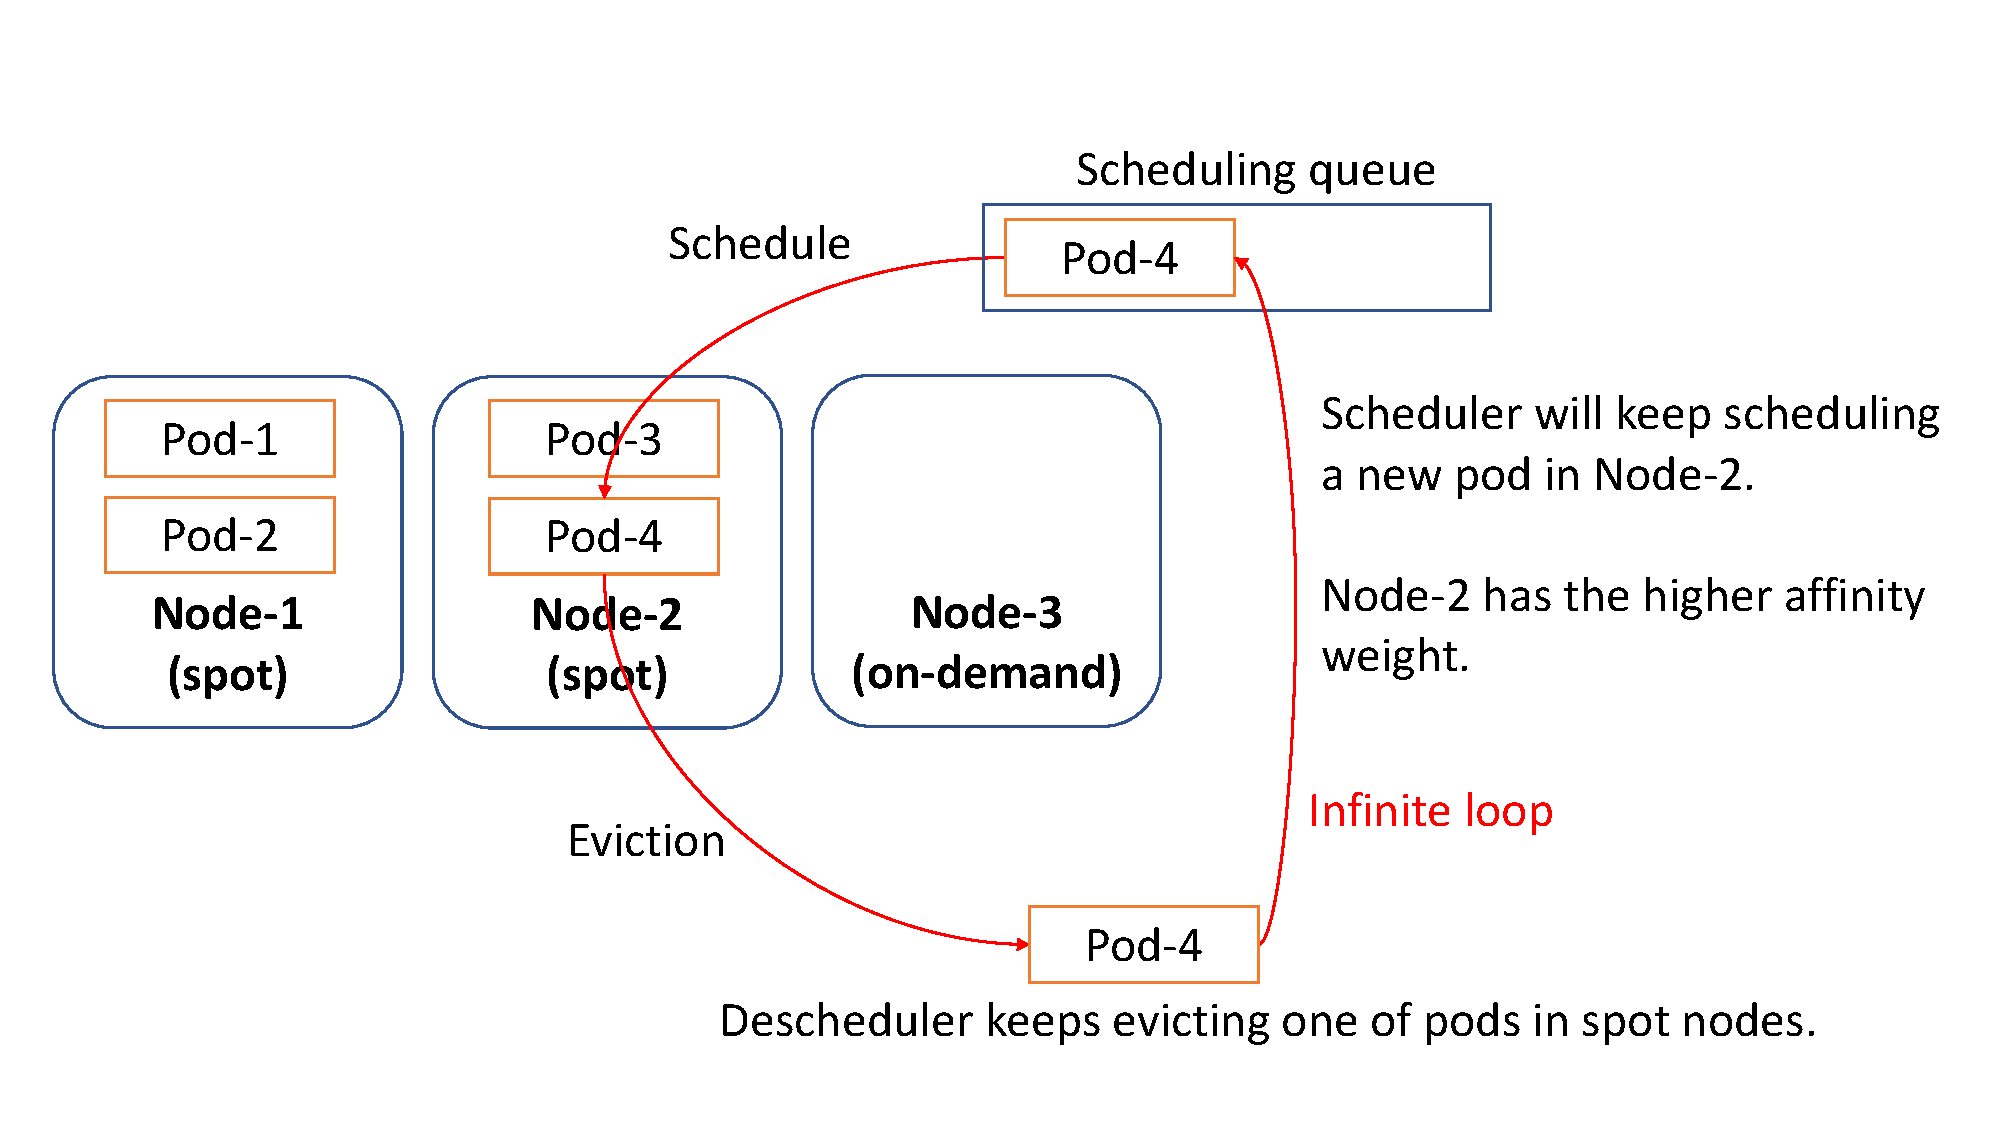
\includegraphics[width=0.5\textwidth]{figure/failure-case-S2.pdf}
    \caption{Failure case S2.}
    \label{fig:s2}
\end{figure}

\subsection*{Failure cases}
In this section, we will walk through 8 failure cases to provide detailed picture of how multi-controller can fall apart. All failure cases are elephant in the room. The problem exists clearly right there in the cluster, nibbling away at cluster resources but none of controllers can recognize it or stop it.  \textit{S3} case will not be described in this paper. It is explained in Kubernetes official document ~\cite{s3_failure}.

\paragraph*{D1, Deployment + Kubelet (Taint)}
Deployment controller~\cite{deployment} manages updates for pods. It has \textit{nodename} configuration which is one way of restricting pods to run in a specific node.
\textit{Kubelet}~\cite{kubelet} is node managment agent. Node can be marked by \textit{Taint} configuration to restrict pods that can be scheduled in the node. Pod is required to have corresponding \textit{Toleration} in order to be schedulable in the tainted node. 
% \textit{NoExecute} taint will not let non-tolerated pods scheduled and already running non-tolerated pods will be all evicted from the node.
The first pathological behavior is triggered if \textit{nodename} in deployment and \textit{Taint} in Kubelet try to do exactly the opposite scheduling. 
For example, deployment specifies \textit{node-1} for explicit pod scheduling.
However, the node is tainted and pod does not have the corresponding toleration.
In this case, two conflicted controllers will create infinite loop of Deployment controller scheduling pods to node-1 and Kubelet controller evicting pods from node-1. Apparently, nothing will stop to form a vicious scheduling cycle. 
Furthermore, \textit{TerminationGracePeriodSeconds} configuration in deployment lets you handle termination gracefully (default: 30s). It can result in a large number of pods in \textit{terminating} status, still taking up cluster resources. 

\paragraph*{H1, HPA + App CPU utilization change}
\textit{Horizontal Pod Autoscaler (HPA)}~\cite{hpa} is in charge of automatically scaling up and down based on defined scaling rule (default: 50\% CPU utilization). If average pod CPU utilization of a deployment exceeds 50\%, HPA will create new pods to satisfy the target metric value. 
HPA does not take into consideration why CPU utilization increases. One common source of increase in CPU utilization could be surge in the number of incoming requests. In this case, scaling up is valid reaction. However, there are other sources of CPU usage. For example, garbage collection, initilization phase of application or any other forms of computation happening inside application are going to increase CPU utilization as well. For these cases, even if scaling up will not help to reduce the CPU utilization, it will scale up since HPA differentiate where CPU increase comes from. Unintended scale up is critical issue, leading to increase in cost. Again, note that none of application and HPA controller is doing anything wrong individually.

\paragraph*{H2, Deployment + HPA}
You can specify the number of replicas in deployment configuration (Default: 1). A deployment is applied with empty replica field and it creates 1 replica. HPA is applied later with configuration of 6 minimum replica and now the number of replicas becomes 6. At some point, you applied a new configuration for the deployment and at this time, the replica field is defined to 3. One of two controllers' replica configuration should be ignored. However, what happens is the number of replicas becomes 3 temporarily for a few seconds by deployment and 6 again by HPA. If the intented number of replica is 6, the change is sub-optimal. If the intent is 3, it fails due to duplicate configuration.

% \paragraph*{H3}

\paragraph*{S1, Scheduler + Descheduler}
Scheduler and Descheduler could be configured to prefer low utiliation node or high utilization node. Default behavior of scheduler is spreading pods as much as it can to make it more fault-tolerant. The purpose of preferring high utilization node is to enable bin packing, retains less number of nodes required to run the cluster and save the overall cost. Unnecessary scheduling and descheduling cycle could be created by confliction between the two controllers. Scheduler is configured to place pods in high utilization node and descheduler is condfigured to evict pods from high utilization node. 

\paragraph*{S2, Daemonset + Descheduler}
\textit{Daemonset} will manage a part of scheduling rule. One of them is \textit{NodeAffinity}. It schedules pods based on affinity weight. The problematic situation is daemonset checks the node affinity and scheduler keeps placing pods in node-1. At the same time, descheduler is running with \textit{RemoveDuplicate} configuration which forces only one pod to run in a node and evicts the rest of them. It is per deployment policy. NodeAffinity and RemoveDuplicate are conflicted each other and will create endless cycle of termination, eviction and creation of pod. 
\textit{S5} arises in a similar fashion by image locality config in deployment and descheduler.

\paragraph*{S6, Node maintenance + Scheduler}
From time to time, nodes could be put in maintenance, for example to add a new library, update security feature. Onec the node is shut down, pods in the node will be terminated and scheduled to another node. For instance, there are three nodes and three replica, one replica running in each node. The node-1 is going through the maintenance and automatically the pod running there is moved to the node-2. The overall placement becomes skewed but it is the best possible movement at the moment. Later, the maintenance finishes and node-1 begins operation again. The expectation is rebalancing the pod spread by moving one pod from node-2 to node-1. Apparently, it will not happen unless descheduler is installed with right plugin (Descheduler is not default controller). This is not the optimal placement and reduces availability by failing appropriate pod spread. 


\paragraph*{S7, Scheduler + Kubelet}
In this failure case, scheduler is configured with maxSkew of 1. Maximum skewness allowed is 1. The deployment creates 3 pods and scheduler will place one pod per a node, pod-\textit{\{1,2,3\}} in node-\textit{\{1,2,3\}} respectively in this example. However, node-3 becomes \textit{NotReady} since kubelet in node-3 is unreponsive for some reason. Pod-3 is not able to be scheduled or will be evicted if it was running. It is expected that node-3 should not be counted when censoring the maxSkew and pod-3 is still scheduled in one node among healty nodes, node-1 and node-2. It does not violate maxSkew:1 rule (two pods in node-1 and one pod in node-2 or the other way around). What actually happens is pod-3 will not be scheduled and remains pending indefinitely since node-3 is still included for maxSkew calculation. It needs to be investigaed further to diagnose the root cause. Regardless of why it occurs, it is counter-intuitive to human that a pod cannot be scheduled due to unresponsive node. It means it is hard to diagnose it when it happens and Kuberentes again does not alert any warning. It is another potential black hole that will suck human resources, wasting their time to look into the issue.
